% -*- TeX -*- -*- UK -*-
% ----------------------------------------------------------------
\documentclass[12pt]{article}
%Preamble:
\usepackage{a4wide}
\input{sl_preamble.tex}
\hypersetup{colorlinks,linkcolor=blue,citecolor=teal,urlcolor=teal}
\input{sl_graphics_preamble.tex}
\graphicspath{{"Figures/"}}
%
\usepackage{array}
\newcounter{tablerow}
\newcommand{\tablerowautorefname}{row}
\newenvironment{tabularn}[1]{\setcounter{tablerow}{0}\begin{tabular}{#1>{\refstepcounter{tablerow}}l}}{\end{tabular}}
%\usepackage{etoolbox}
%\AtBeginEnvironment{tabular}{\setcounter{tablerow}{0}}
%
% ----------------------------------------------------------------
% New commands etc.
\input{sl_definitions.tex}
\input{sl_symbols.tex}
%matrices
\newcommand{\I}{\mathbf{I}}
%vec of ones
%equilibrium distribution
\newcommand{\pr}{\mathbf{p}}
\newcommand{\eq}{\pr^\infty}
%other symbols
\newcommand{\w}{\mathbf{w}}
\newcommand{\W}{\mathbf{W}}
\newcommand{\frg}{\W^\mathrm{F}}
\newcommand{\M}{\mathbf{M}}
\newcommand{\F}{\boldsymbol{\Phi}}
\newcommand{\pot}{^{\text{pot}}}
\newcommand{\dep}{^{\text{dep}}}
\newcommand{\potdep}{^{\text{pot/dep}}}
\newcommand{\norm}{_0}
\newcommand{\inc}{_{\text{inc}}}
\newcommand{\dec}{_{\text{dec}}}
\newcommand{\incdec}{_{\text{inc/dec}}}
\newcommand{\wt}{_{\text{WT}}}
\newcommand{\ko}{_{\text{D$^\mathrm{b}$K$^\mathrm{b}$-/-}}}
\newcommand{\KO}{D$^\mathrm{b}$K$^\mathrm{b}$-/-}
\newcommand{\tpre}{t_{\text{pre}}}
\newcommand{\ttrain}{t_{\text{train}}}
\newcommand{\lmax}{_{\text{max}}}
\newcommand{\lmin}{_{\text{min}}}
% ----------------------------------------------------------------
%
%%%%%%%%%%%%%%%%%%%%%%%%%%%%%%%%%%%%%%%%%%%%%%%%%%%%%%%%%%%%%%%%%%%%%%%%%%
% Title info:
\title{A saturation model for impaired learning with enhanced plasticity: Supplementary material}
%
%% Author List:
%%
%\author{An Author$^a$, Another Author$^b$ and Yet Another Author$^c$\\
%%
%\small{\emph{$^a$ Address 1}}\\
%\small{\emph{$^b$ Address 2}}\\
%\small{\emph{$^c$ Address 3}}\\
%}

\begin{document}

\maketitle


%%%%%%%%%%%%%%%%%%%%%%%%%%%%%%%%%%%%%%%%%%%%%%%%%%%%%%%%%%%%%%%%%%%%%%%%%%


%\begin{abstract}
%  We see if we can model VOR gain increase and decrease learning in mice with a knockout in MHC as well as wild-type.
%\end{abstract}

\tableofcontents
\listoffigures

%%%%%%%%%%%%%%%%%%%%%%%%%%%%%%%%%%%%%%%%%%%%%%%%%%%%%%%%%%%%%%%%%%%%%%%%%%
% Beginning of Article:
%%%%%%%%%%%%%%%%%%%%%%%%%%%%%%%%%%%%%%%%%%%%%%%%%%%%%%%%%%%%%%%%%%%%%%%%%%

\section{Mathematical formalism}\label{sec:setup}


\subsection{Models of synapses}\label{sec:synapse}

We make the following assumptions:
\begin{itemize}
  \item There are $N$ identical synapses with $M$ internal functional states.
  \item The states of different synapses are independent of each other.
  \item The synapses that are eligible for plasticity are chosen randomly.
  \item The potentiating/depressing plasticity event timings are distributed as Poisson processes with rates $rf\potdep$, where $f\pot+f\dep=1$.
      In other words, $r$ is the total rate of plasticity events per synapse and $f\potdep$ are the fraction of these events that are potentiating/depressing.
  \item Potentiation and depression are described by Markov processes with transition probabilities $\M\potdep$.
  \item The synaptic weights of the internal states are given by the column vector $\w$. This can only take values in a finite range that we can shift to $\pm1$. Most of the models will only use the two extreme values.
\end{itemize}

The independence and identicalness of synapses means that the state of the system can be completely described by the probability distribution of the internal states, the row vector $\pr(t)$.

The evolution of this probability is described by a forgetting matrix, $\frg$:
%
\begin{equation}\label{eq:evolve}
  \diff{\pr(t)}{t} = r\pr(t)\frg,
  \qquad
  \frg = f\pot\M\pot+f\dep\M\dep-\I,
\end{equation}
%
where $\I$ is the identity matrix.
Eventually, this will settle into the equilibrium distribution:
%
\begin{equation}\label{eq:eqprob}
  \eq\frg=0.
\end{equation}
%

For models with only two possible synaptic weights, the distribution of synaptic weights is completely described by the mean, $\pr(t)\w$.


The MHC mutant has a lower threshold for depression.
We can model this by changing $\M\dep\wt$ to $\M\dep\ko$, which should have larger off-diagonal matrix elements.

We will look at several different models,
the multistate model\footnote{The original definition of the multistate model had a synaptic weight that varied linearly along the chain. We will refer to this as the linear multistate model. We will also look at the step-multistate model, for which the synaptic weight takes only two values.} (see \cite{amit1994learning,Fusi2007multistate} and \autoref{fig:models}\ref{fig:multistate_model}),
the two-state model (which can be thought of as a special case of the multistate model, see \autoref{fig:models}\ref{fig:binary_model}),
and the cascade model (see \cite{Fusi2005cascade} and \autoref{fig:models}\ref{fig:cascade_model}).
We will also look at a new, pooled resource model that we will define below in \autoref{sec:pooledmodel}.

For the multistate and two state models, we will use the same value for the transition probabilities, $q$, for potentiation and depression in the wild-type as well as potentiation in the \KO\ mutant.
We will use a larger value for $q$ for depression in the \KO\ mutant.

For the cascade model, we will use the same value for the parameter $x$ (which controls the decay of transition rates, see \cite{Fusi2005cascade}) for potentiation and depression in the wild-type as well as potentiation in the \KO\ mutant.
We will use a larger value for $x$ for depression in the \KO\ mutant.

The values used for all these parameters in simulations are listed in \autoref{tab:params}.

\begin{figure}
 \begin{center}
 \begin{myenuma}
  \item\aligntop{\includegraphics[height=1.7cm]{multistate.svg}}\label{fig:multistate_model}\hspace{0.5cm}
  \item\aligntop{\includegraphics[height=1.7cm]{binary.svg}}\label{fig:binary_model}\hspace{0.5cm}
  \item\aligntop{\includegraphics[height=2.2cm]{cascade.svg}}\label{fig:cascade_model}
 \end{myenuma}
 \end{center}
  \caption[Transition probabilities for different models]{Transition probabilities for different models.
  Potentiation induces transitions indicated by solid red arrows, depression indicated by dashed blue arrows.
  States of strong/weak synaptic weight indicated by red/blue circles.
  States of strong/weak synaptic weight
  (\ref{fig:multistate_model}) In the multistate model the transition probabilities for potentiation/depression are all equal and it is parameterised by these two values.
  (\ref{fig:binary_model}) The two-state model is parameterised by the two transition probabilities.
  (\ref{fig:cascade_model}) In the cascade model, the transition probabilities decay geometrically with a parameter $x$ (see \cite{Fusi2005cascade}) and synaptic weight takes only two values.
  } \label{fig:models}
\end{figure}

\subsubsection{Pooled resource model}\label{sec:pooledmodel}

Suppose that there is some resource required for potentiation/depression that is shared between $P$ synapses and is depleted as more synapses are potentiated/depressed and replenished when this is reversed.
We can avoid going beyond the independent synapse model by modelling this pool of synapse as a single compound synapse.

We will model the individual synapses with the two-state model.
Let $i=0\ldots P$ be the number of them that are potentiated.
We will model the effect of resource depletion linearly with the potentiation/depression probabilities for the individual synapses:
%
\begin{equation}\label{eq:depletion}
  \begin{aligned}
    q\pot &= \frac{(P-i-1)q\lmax + i\,q\lmin}{P-1}, \quad& i &= 0 \ldots P-1,\\
    q\dep &= \frac{(i-1)q\lmax + (P-i)q\lmin}{P-1}, & i &= 1 \ldots P.
  \end{aligned}
\end{equation}
%
At each plasticity event for the compound synapse, one of the individual synapses will be chosen randomly for update.
This effectively reduces the transition probabilities by $1/P$.

This compound synapse would seem to have $2^P$ internal states.
However, we need only keep track of the number of potentiated synapses, not their identity, leaving $M=P+1$ states.
The transition network will then have a multistate topology (see \autoref{fig:models}\ref{fig:multistate_model}) but the transition probabilities will no longer be uniform and the weight of the compound synapse is the mean of its constituent synapses:
%
\begin{equation}\label{eq:pooledweight}
  \w_i = \frac{2i}{P}-1.
\end{equation}
%


The Markov process is lumpable \wrt this partition of states (see \cite[\S6.3]{kemeny1960finite} for the discrete time version and \cite{burke1958markovian,Ball1993Lumpability} for continuous time).
The transition probabilities between lumps $i$ and $j$ is computed by choosing one state from lump $i$ and summing the transition probabilities to all states in lump $j$.
The result must be the same for all states in lump $i$.

For any state in lump $i$, there are $P-i$ synapses that can be potentiated to go to lump $i+1$.
Each of these transition probabilities is $q\pot/P$.
Similarly, there are $i$ synapses that can be depressed to go to lump $i-1$.
Each of these transition probabilities is $q\dep/P$.
Thus:
%
\begin{equation}\label{eq:pooledpotdep}
  \begin{aligned}
    \M\pot_{ii+1} &=  \brk{\frac{(P-i-1)q\lmax + i\,q\lmin}{P-1}} \frac{P-i}{P} ,
      \quad& i &= 0 \ldots P-1,\\
    \M\dep_{ii-1} &=  \brk{\frac{(i-1)q\lmax + (P-i)q\lmin}{P-1}} \frac{i}{P} ,
           & i &= 1 \ldots P,
  \end{aligned}
\end{equation}
%
with all other off-diagonal elements equal to zero.
The diagonal elements are chosen so that the rows sum to one.

This model is parameterised by the range of values, $q\in[q\lmin,q\lmax]$, for potentiation and depression.
We will use the same values for potentiation and depression in the wild-type as well as potentiation in the \KO\ mutant.
We will use larger values for depression in the \KO\ mutant.
The values of these parameters are listed in \autoref{tab:params}.


\begin{figure}
 \begin{center}
  \aligntop{\includegraphics[height=4cm]{pooled.svg}}
 \end{center}
  \caption[The pooled resource model]{The pooled resource model.
  Several two-state synapses share resources that are required for potentiation and depression.
  These resources are depleted as more synapses are potentiated or depressed.
  This pool of synapses can be modelled as one compound synapse.} \label{fig:pooled_model}
\end{figure}



\subsection{Model of VOR learning experiment}\label{sec:learning}

Training the animal will not change the internal dynamics of a synapse under potentiation or depression.
It will change the environment, which will lead to a change in how often potentiation and depression occur.
It could be manifested in a change in which synapses are potentiated/depressed, but this could not be captured in this type of model.
We will model this by changing $f\potdep$, leaving $r$ and $\M\potdep$ unchanged.

The untrained case will be described by $f\pot=f\pot\norm$.
Gain-increase training  will be described by $f\pot=f\pot\inc<f\pot\norm$, and
gain-decrease training  will be described by $f\pot=f\pot\dec>f\pot\norm$. Note that the forgetting matrix \eqref{eq:evolve} and the equilibrium distribution \eqref{eq:eqprob} depend on $f\pot$, which we will indicate with subscripts.

Before training, the synaptic distribution will be in the equilibrium distribution corresponding to $f\pot\norm$.
During gain-increase training, it will evolve according to \eqref{eq:evolve} with $f\pot\inc$:
%
\begin{equation}\label{eq:nopre}
  \pr(t) = \eq\norm \exp\prn{rt\frg\inc}.
\end{equation}
%
On the other hand, if the gain-increase training follows gain-decrease pre-training for some time period, $\tpre$:
%
\begin{equation}\label{eq:withpre}
  \pr(t) = \eq\norm \exp\prn{r\tpre\frg\dec} \exp\prn{r(t-\tpre)\frg\inc}.
\end{equation}
%

We will describe the effect of training by the decrease in mean synaptic weight:
%
\begin{equation}\label{eq:learning}
  L(t) = \prn{\pr(0)-\pr(t)}\w.
\end{equation}
%
If we imagine something like an LN model for the Purkinje cell, the output would depend on some linear combination of the synaptic weights (weighted by the activities of the corresponding parallel fibres).
If we're not keeping track of synaptic identity, the most natural linear combination to use would be an equal sum of them all.
The behavioural output (VOR gain) will be some unknown, non-linear function of the synaptic weights, so the best we can hope for is to reproduce qualitative features of the experiment, such as whether learning is enhanced or impaired by the mutation or pre-training.

We will assume $f\pot\wt=f\pot\ko$.
This is because the mutation is well localised to the Purkinje cells, so the activity of the parallel and climbing fibres should not change very much.
Therefore the rates of potentiation and depression should not change very much either.
This implies that the mean synaptic weight in equilibrium differs between the mutant and wild type, but that is also suggested by the data regarding basal levels of phospho-GluR2 at serine 880.
As the mutation produces no change in baseline performance, there must be a compensatory mechanism somewhere else.
We will model this compensation as a simple linear offset, as could be produced by another population of neurons/synapses whose effect cancels with these neurons/synapses.

For the most part, we set $f\pot\norm=\half$, $f\pot\inc=f\pot\norm+\Delta f$ and $f\pot\dec=f\pot\norm-\Delta f$, with $\Delta f<0$.
We use the same values for wild-type and mutant and treat gain-increase and decrease symmetrically.
The values of these parameters are listed in \autoref{tab:params}.

We are also assuming that the relation between VOR gain and mean synaptic weight is the same for mutant ant wild-type, except for a linear offset to compensate for the difference in equilibrium weights mentioned above.
This ensures that the qualitative questions mentioned above (enhancement or impairment of learning) will not be affected.




\section{Simulation and analysis of models}\label{sec:results}

The features of the actual experiments that we'd like to capture are:
\begin{enumerate}
  \item Without pre-training, gain-increase learning is significantly faster in the wild-type than in the mutant.
  \item For the wild-type, gain-increase learning is significantly faster without pre-training than with it.
  \item For the mutant, gain-increase learning is significantly faster with pre-training than without it.
  \item After pre-training, gain-increase learning is significantly faster in the mutant than in the wild-type.
  \item Gain-decrease pre-training is slightly faster in the wild-type, but not significantly so.\label{it:gaindown}
\end{enumerate}
These questions will not be affected by any output nonlinearity, as long as it is monotonic and fixed.
We will not worry too much about \autoref{it:gaindown}, as gain-decrease learning uses a different mechanism to gain-increase.
We are only modelling the effect of gain-decrease training on \emph{these} synapses.

We will not worry too much about the curvature of the learning curves, as this can be changed by the nonlinear relation between synaptic weight and VOR gain.
However, both the wild-type and mutant should be affected in the same way, so the difference in the curvature of the mutant and wild-type curves after pre-training would be nice to capture.

We will try to gain some analytic insight to some of these models by looking at the slope of the learning curve at the start of gain-increase training.
This is proportional to the net-flux from the states with strong synaptic weight to the weaker states, measured using the transition probabilities for gain-increase but the equilibrium distribution for either untrained or gain-decrease, assuming that pre-training lasts long enough to reach the equilibrium distribution for gain-decrease.
This should be multiplied by the difference in synaptic weights.
But, as this quantity is constant within a model and doesn't change when comparing wild-type and mutant or with/without pre-training, it can be ignored.

The values for all parameters we will use can be found in \autoref{tab:params}.


\begin{table}
 \begin{center}
  \begin{tabularn}{|l|c|c|c|c|c|c|}
    \cline{1-7}
    % after \\: \hline or \cline{col1-col2} \cline{col3-col4} ...
    Model & \# states & pot,WT dep & \KO\ dep & $\Delta f$ & $r\ttrain$ & $r\tpre$ \\
    \cline{1-7}
    Cascade       & 10 & $x=0.25$ & $x=0.33$ & -0.3  & 50 & 50  &\label{tr:cascade_short} \\
    Cascade       & 10 & $x=0.25$ & $x=0.33$ & -0.3  & 50 & 150 &\label{tr:cascade_long} \\
    Step-multistate    & 10 & $q=0.6$  & $q=0.8$  & -0.1  & 50 & 50  &\label{tr:multistate_weak} \\
    Step-multistate    & 10 & $q=0.6$  & $q=0.8$  & -0.17 & 10 & 30  &\label{tr:multistate_med} \\
    Step-multistate    & 10 & $q=0.6$  & $q=0.8$  & -0.4  & 20 & 20  &\label{tr:multistate_strong} \\
    Linear Multistate & 10 & $q=0.6$  & $q=0.8$  & -0.3  & 20 & 20  &\label{tr:multistate_lin} \\
    Two-state     & 2  & $q=0.4$  & $q=0.8$  & -0.1  & 5  & 5   &\label{tr:binary} \\
    Pooled        & 10 & $q\in[0.3,0.4]$  & $q\in[0.6,0.8]$
                                          & -0.1 & 70 & 70 &\label{tr:pooled_plenty}\\
    Pooled        & 10 & $q\in[0.1,0.4]$  & $q\in[0.2,0.8]$
                                          & -0.1 & 70 & 70 &\label{tr:pooled_scarce}\\
    \cline{1-7}
%   \hline
%    % after \\: \hline or \cline{col1-col2} \cline{col3-col4} ...
%    & Model & \# states & pot,WT dep & \KO\ dep & $\Delta f$ & $r\ttrain$ & $r\tpre$ \\
%    \cline{1-7}
%    \label{tr:cascade_short}&
%    Cascade    & 10 & $x=0.25$ & $x=0.33$ & -0.3 & 50 & 50   \\
%    \label{tr:cascade_long}&
%    Cascade    & 10 & $x=0.25$ & $x=0.33$ & -0.3 & 50 & 150  \\
%    \label{tr:multistate_weak}&
%    Multistate & 10 & $q=0.6$  & $q=0.8$  & -0.1 & 50 & 50   \\
%    \label{tr:multistate_strong}&
%    Multistate & 10 & $q=0.6$  & $q=0.8$  & -0.4 & 20 & 20   \\
%    \label{tr:binary}&
%    Two-state  & 2  & $q=0.4$  & $q=0.8$  & -0.1 & 5  & 5    \\
%    \label{tr:pooled_plenty}&
%    Pooled     & 10 & $q\in[0.3,0.4]$  & $q\in[0.6,0.8]$
%                                          & -0.1 & 70 & 70 \\
%    \label{tr:pooled_scarce}&
%    Pooled     & 10 & $q\in[0.1,0.4]$  & $q\in[0.2,0.8]$
%                                          & -0.1 & 70 & 70 \\
%    \cline{1-7}
  \end{tabularn}
 \end{center}
  \caption{Parameters used in simulations.} \label{tab:params}
\end{table}


\newcommand{\resultsfig}[3]{\begin{figure}
 \begin{center}
 \begin{myenuma}
  \item\aligntop{\includegraphics[width=7cm]{#3_learn.eps}}\label{fig:#3_learn}
  \item\aligntop{\includegraphics[width=7cm]{#3_learnS.eps}}\label{fig:#3_learnS}
  \\ \vp\vp
  \item\label{fig:#3_eq}\begin{myenumi}
                    \item\aligntop{\includegraphics[width=7cm]{#3_eq_WT.eps}}\label{fig:#3_eq_WT}
                    \item\aligntop{\includegraphics[width=7cm]{#3_eq_KO.eps}}\label{fig:#3_eq_KO}
                  \end{myenumi}
  \\ \vp \vp
  \item\label{fig:#3_pr}\begin{myenumi}
                    \item\aligntop{\includegraphics[width=3cm]{#3_pr_WT_nopre.eps}}\label{fig:#3_pr_WT_nopre}
                    \item\aligntop{\includegraphics[width=3cm]{#3_pr_WT_pre.eps}}\label{fig:#3_pr_WT_pre}
                    \item\aligntop{\includegraphics[width=3cm]{#3_pr_KO_nopre.eps}}\label{fig:#3_pr_KO_nopre}
                    \item\aligntop{\includegraphics[width=3cm]{#3_pr_KO_pre.eps}}\label{fig:#3_pr_KO_pre}
                  \end{myenumi}
 \end{myenuma}
 \end{center}
  \caption[#1]{#1 #2.
  Other parameters can be found in \autoref{tr:#3} of \autoref{tab:params}.
  Time is measured in units of $1/r$, the mean time between plasticity events.
  (\ref{fig:#3_learn}) Learning curves for wild-type and \KO\ mutant with and without pre-training.
  (\ref{fig:#3_learnS}) Learning curves restricted to gain-increase training.
  (\ref{fig:#3_eq}) Equilibrium distributions without training or with gain-increase/decrease training for (\ref{fig:#3_eq_WT}) wild-type and (\ref{fig:#3_eq_KO}) \KO\ mutant,
  with states of weak synaptic strength to the left and strong states to the right.
  (\ref{fig:#3_pr}) Evolution of probability distributions for (\ref{fig:#3_pr_WT_nopre}\ref{fig:#3_pr_WT_pre}) wild-type and  (\ref{fig:#3_pr_KO_nopre}\ref{fig:#3_pr_KO_pre}) \KO\ mutant without (\ref{fig:#3_pr_WT_nopre},\ref{fig:#3_pr_KO_nopre}) and with (\ref{fig:#3_pr_WT_pre},\ref{fig:#3_pr_KO_pre}) pre-training,
  with states of weak synaptic strength at the top and strong states underneath. } \label{fig:#3}
\end{figure}}

\newcommand{\resultsfign}[2]{\begin{figure}
 \begin{center}
 \begin{myenuma}
  \item\aligntop{\includegraphics[width=7cm]{#2_learn.eps}}\label{fig:#2_learn}
  \item\aligntop{\includegraphics[width=7cm]{#2_learnS.eps}}\label{fig:#2_learnS}
  \\ \vp \vp
  \item\label{fig:#2_eq}\begin{myenumi}
                    \item\aligntop{\includegraphics[width=7cm]{#2_eq_WT.eps}}\label{fig:#2_eq_WT}
                    \item\aligntop{\includegraphics[width=7cm]{#2_eq_KO.eps}}\label{fig:#2_eq_KO}
                  \end{myenumi}
  \\ \vp \vp
  \item\label{fig:#2_pr}\begin{myenumi}
                    \item\aligntop{\includegraphics[width=3cm]{#2_pr_WT_nopre.eps}}\label{fig:#2_pr_WT_nopre}
                    \item\aligntop{\includegraphics[width=3cm]{#2_pr_WT_pre.eps}}\label{fig:#2_pr_WT_pre}
                    \item\aligntop{\includegraphics[width=3cm]{#2_pr_KO_nopre.eps}}\label{fig:#2_pr_KO_nopre}
                    \item\aligntop{\includegraphics[width=3cm]{#2_pr_KO_pre.eps}}\label{fig:#2_pr_KO_pre}
                  \end{myenumi}
 \end{myenuma}
 \end{center}
  \caption[#1]{#1.
  Parameters can be found in \autoref{tr:#2} of \autoref{tab:params}.
  Time is measured in units of $1/r$, the mean time between plasticity events.
  (\ref{fig:#2_learn}) Learning curves for wild-type and \KO\ mutant with and without pre-training.
  (\ref{fig:#2_learnS}) Learning curves restricted to gain-increase training.
  (\ref{fig:#2_eq}) Equilibrium distributions without training or with gain-increase/decrease training for (\ref{fig:#2_eq_WT}) wild-type and (\ref{fig:#2_eq_KO}) \KO\ mutant,
  with states of weak synaptic strength to the left and strong states to the right.
  (\ref{fig:#2_pr}) Evolution of probability distributions for (\ref{fig:#2_pr_WT_nopre}\ref{fig:#2_pr_WT_pre}) wild-type and  (\ref{fig:#2_pr_KO_nopre}\ref{fig:#2_pr_KO_pre}) \KO\ mutant without (\ref{fig:#2_pr_WT_nopre},\ref{fig:#2_pr_KO_nopre}) and with (\ref{fig:#2_pr_WT_pre},\ref{fig:#2_pr_KO_pre}) pre-training,
  with states of weak synaptic strength at the top and strong states underneath. } \label{fig:#2}
\end{figure}}



\subsection{Step-multistate model}\label{sec:multistate}

\resultsfig{Simulation results for the step-multistate model with weak training}{($\Delta f=-0.1$)}{multistate_weak}

\resultsfig{Simulation results for the step-multistate model with moderate training}{($\Delta f=-0.17$)}{multistate_med}

\resultsfig{Simulation results for the step-multistate model with strong training}{($\Delta f=-0.4$)}{multistate_strong}


The results of simulations of the step-multistate model can be seen in \autoref{fig:multistate_weak}, \autoref{fig:multistate_med} and \autoref{fig:multistate_strong}.
However, we can get some insight into this model analytically.



Consider the general uniform multistate model.
Then the equilibrium distribution is given by
%
\begin{equation}\label{eq:mutltieq}
  \eq_i = \frac{1-\alpha}{1-\alpha^M}\,\alpha^{i-1},
  \qquad \text{where} \quad
  \alpha=\frac{f\pot q\pot}{f\dep q\dep}.
\end{equation}
%
If we take the limit $\alpha\rightarrow1$, this becomes $\frac{1}{M}$.

The net-flux from the $\w=+1$ states to the $\w=-1$ states is:
%
\begin{equation}\label{eq:multiflux}
  \Phi = \eq_{M/2+1}f'{}\dep q\dep - \eq_{M/2}f'{}\pot q\pot = \frac{1-\alpha}{1-\alpha^M}\,\alpha^{M/2-1}\prn{\alpha-\alpha'}f'{}\dep q\dep,
\end{equation}
%
where primed values correspond to the new value of $f\pot$.

First, consider the wild-type, for which $q\pot=q\dep=q$.
Without pre-training:
%
\begin{equation}\label{eq:multiWTnopre}
  \Phi = \frac{2\abs{\Delta f}q}{M},
\end{equation}
%
where it's worth remembering that $\Delta f<0$.
With pre-training:
%
\begin{equation}\label{eq:multiWTpre}
\begin{aligned}
  \Phi &= 16(\Delta f)^2q \, \frac{(1-2\Delta f)^{M/2-1} (1+2\Delta f)^{M/2-1}}
          {(1-2\Delta f)^M - (1+2\Delta f)^M} \\
       &= \frac{4\abs{\Delta f}q}{M} + \CO(\Delta f)^2.
\end{aligned}
\end{equation}
%
So, we see that pre-training will speed up learning when $\Delta f$ is small (in absolute value), as seen in \autoref{fig:multistate_weak}\ref{fig:multistate_weak_learnS} (black curves).
On the other hand, if $\Delta f$ is close to $-\half$, pre-training will initially slow down learning a lot due to the factor of $(1+2\Delta f)^{M/2-1}$, as seen in \autoref{fig:multistate_strong}\ref{fig:multistate_strong_learnS}.

Intuitively, the flux depends on the slope of the distribution at the centre of the chain (with an offset due to the difference between $f\pot$ and $f\dep$).
Pre-training has two effects: it produces a slope in the right direction (see \autoref{fig:multistate_weak}\ref{fig:multistate_weak_eq}, red trace), but it also reduces the distribution at the centre (see \autoref{fig:multistate_strong}\ref{fig:multistate_strong_eq}, red trace).
For small $\Delta f$, the first effect is stronger and learning speeds up.
For larger $\Delta f$, the second effect wins and learning slows down.

Now, consider the mutant, for which $q\pot=\beta q\dep=q$, $\beta<1$.
Without pre-training:
%
\begin{equation}\label{eq:multiKOnopre}
  \Phi = 2\abs{\Delta f} q\,\frac{(1-\beta)\beta^{M/2-1}}{1-\beta^M}.
\end{equation}
%
This will be smaller than \eqref{eq:multiWTnopre} if $\beta<\beta^*(M)$.
This function is plotted in \autoref{fig:multistate_star}\ref{fig:multistate_betastar}, where we can see that it approaches 1 rapidly as we increase $M$.

There are two effects here as well.
Smaller $\beta$ will increase the probability of crossing the centre of the chain, speeding up learning, but it will also concentrate probability at the ends of the chain, depleting the centre and slowing down learning (see \autoref{fig:multistate_strong}\ref{fig:multistate_strong_eq}\ref{fig:multistate_strong_eq_KO}, blue trace).
The first effect goes like $1/\beta$, whereas the second goes like $\beta^{M/2}$ and will be more significant for smaller $\beta$ or in a longer chain.

With pre-training:
%
\begin{equation}\label{eq:multiKOpre}
\begin{aligned}
  \Phi &= 4\abs{\Delta f} q \, \frac{(1+2\Delta f) - \beta(1-2\Delta f)}
          {(1+2\Delta f)^M - \beta^M(1-2\Delta f)^M}   \,
          \brk{\beta (1-2\Delta f) (1+2\Delta f)}^{M/2-1} \\
       &= 4\abs{\Delta f} q\,\frac{(1-\beta)\beta^{M/2-1}}{1-\beta^M} + \CO(\Delta f)^2.
\end{aligned}
\end{equation}
%
Once again, we see that pre-training will speed up learning when $\Delta f$ is small, whereas, if $\Delta f$ is close to $-\half$, pre-training will initially slow down learning.

Let us define $\Delta f^*(\beta,M)$ to be the value at which \eqref{eq:multiKOnopre} and \eqref{eq:multiKOpre} are equal.
Values of $\Delta f$ that are smaller than this (stronger training) will correspond to slower learning after pre-training.
As we would like pre-training to slow down learning in the wild-type but speed it up in the mutant, it would seem that we require $\Delta f^*(\beta,M) < \Delta f < \Delta f^*(1,M)$ (remembering once more that $\Delta f<0$ and that the wild-type corresponds to $\beta=1$).
As we see in \autoref{fig:multistate_star}\ref{fig:multistate_deltafstar}, $\Delta f^*(\beta,M) < \Delta f^*(1,M)$, so this range always exists.
We can see an example of this in \autoref{fig:multistate_med}\ref{fig:multistate_med_learnS}.

However, this is only the initial, instantaneous rate of change.
Let's look at \autoref{fig:multistate_strong}\ref{fig:multistate_strong_learnS}, for which $\Delta f < \Delta f^*(1,M)$, so that pre-training initially slows down learning for both wild-type and mutant.
We see that the pre-trained curve can rapidly catch up with the un-pre-trained one, due to the mass of probability concentrated at the end of the chain (see \autoref{fig:multistate_strong}\ref{fig:multistate_strong_eq}, red trace) drifting to the centre.
This happens sooner for the mutant than the wild-type, due to the stronger depressing transitions.
This means that there is an intermediate range of time-scales over which pre-training does slow down learning in the wild-type but speed it up in the mutant, even outside the desired range of values for $\Delta f$.
As we see in \autoref{fig:multistate_med}\ref{fig:multistate_med_learnS} (black curves), even when we are in this range, the period of time for which pre-training impairs learning in the wild-type can be very small.

\begin{figure}
 \begin{center}
 \begin{myenuma}
  \item\aligntop{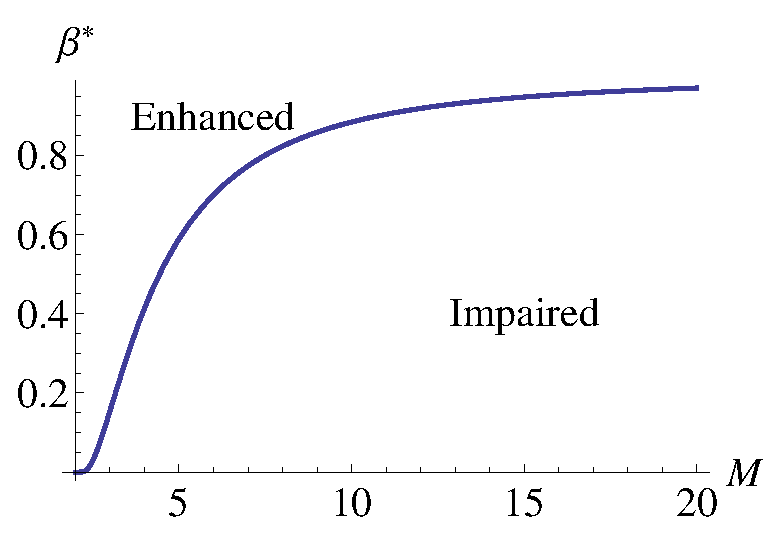
\includegraphics[width=7cm]{multistate_betastar.eps}}\label{fig:multistate_betastar}
  \item\aligntop{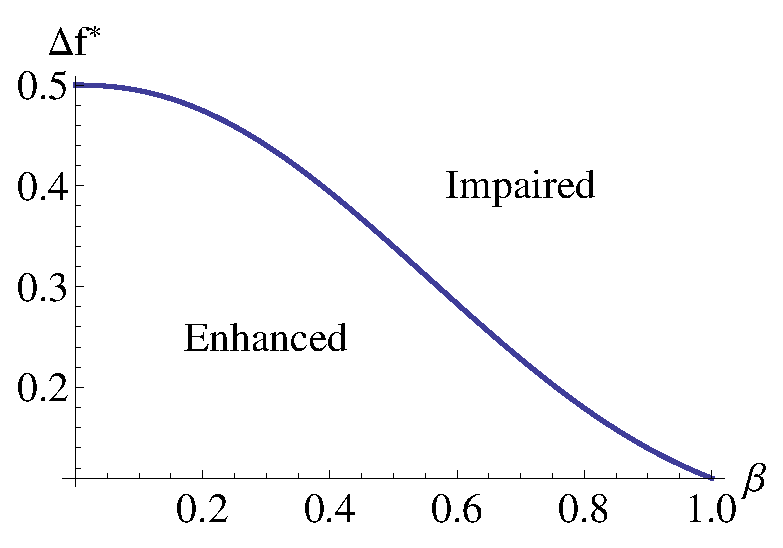
\includegraphics[width=7cm]{multistate_deltafstar.eps}}\label{fig:multistate_deltafstar}
 \end{myenuma}
 \end{center}
  \caption[The functions $\beta^*(M)$ and $\Delta f^*(\beta,M)$]{The functions (\ref{fig:multistate_betastar}) $\beta^*(M)$, which describes when the mutant has impaired learning, and (\ref{fig:multistate_deltafstar}) $\Delta f^*(\beta,M)$ for $M=10$, which describes when pre-training enhances learning.}\label{fig:multistate_star}
\end{figure}

In conclusion, if we choose $\beta<\beta^*(M)$, $\Delta f < \Delta f^*(1,M)$ and look at intermediate time-scales, we will see that the mutant learns slower than wild-type without pre-training, and that pre-training speeds up learning in the mutant but slows it down in the wild-type.
However, in this case pre-training proceeds much faster in the mutant than wild-type (see \autoref{fig:multistate_med}\ref{fig:multistate_med_learn} and \autoref{fig:multistate_strong}\ref{fig:multistate_strong_learn}, lower curves), which is \emph{not} seen in the experiment.

Now consider what would happen if we did not treat gain-increase and gain-decrease symmetrically.
Let us set $f\pot\dec = f\pot\norm - \overline{\Delta f}$.
Then, \eqref{eq:multiKOpre} becomes
%
\begin{equation}\label{eq:multiKOdiffpre}
\begin{aligned}
  \Phi &= 2\abs{\Delta f + \overline{\Delta f}} q \, \frac{(1+2\overline{\Delta f}) - \beta(1-2\overline{\Delta f})}
          {(1+2\overline{\Delta f})^M - \beta^M(1-2\overline{\Delta f})^M}   \,
          \brk{\beta (1-2\overline{\Delta f}) (1+2\overline{\Delta f})}^{M/2-1} \\
       &= 2\abs{\Delta f + \overline{\Delta f}} q\,\frac{(1-\beta)\beta^{M/2-1}}{1-\beta^M} + \CO(\Delta f,\overline{\Delta f})^2.
\end{aligned}
\end{equation}
%
We can then look at the wild-type by setting $\beta=1$:
%
\begin{equation}\label{eq:multiWTdiffpre}
\begin{aligned}
  \Phi &= 8\,\overline{\Delta f}\prn{\Delta f + \overline{\Delta f}} q \,
          \frac{(1-2\overline{\Delta f})^{M/2-1} (1+2\overline{\Delta f})^{M/2-1} }
          {\abs{(1+2\overline{\Delta f})^M - (1-2\overline{\Delta f})^M}}   \\
       &= \frac{2\abs{\Delta f + \overline{\Delta f}} q}{M} + \CO(\Delta f,\overline{\Delta f})^2.
\end{aligned}
\end{equation}
%

We can see from these formulae that, if we want pre-training to impair learning in wild-type, but enhance it in the mutant, the important thing is to have \emph{strong pre-training}, not strong training.
Thus, removing the symmetry between gain-increase and gain-decrease will not help with the most unrealistic feature of this model -- the fact that pre-training proceeds much faster in the mutant than wild-type.

Finally, we note that, in the case of medium or strong pre-training, we see positive curvature in the learning curve after pre-training for a longer time in wild-type than in the mutant (see \autoref{fig:multistate_med}\ref{fig:multistate_med_learnS} and \autoref{fig:multistate_strong}\ref{fig:multistate_strong_learnS}, dashed curves).
This is due to the mass of probability at the right end of the chain (see \autoref{fig:multistate_med}\ref{fig:multistate_med_eq} and \autoref{fig:multistate_strong}\ref{fig:multistate_strong_eq}, red trace) that is unable to contribute to change in synaptic weight until it has drifted to the centre.
This will last for a shorter time in the mutant, due to the enhanced transitions.
This will not be a feature of any of the other models that we study here.
Now, the curvature can be changed by the nonlinear relation between synaptic weight and VOR gain, but both curves would be affected in the same way.
The difference in these two curvatures is therefore a good feature of this model.


\subsection{Two-state model}\label{sec:binary}


\resultsfign{Simulation results for two-state model}{binary}


The results of simulations of the two-state model can be seen in \autoref{fig:binary}.
However, this model can be solved exactly:
%
\begin{multline}\label{eq:binarysol}
  \eq = \frac{(f\dep q\dep, f\pot q\pot)}{\lambda},
  \qquad
  \pr(t) = \eq + (\pr(t)-\eq)\e^{-\lambda rt},\\
  \qquad \text{where} \quad
  \lambda = f\pot q\pot + f\dep q\dep.
\end{multline}
%
But it is easier to just substitute $M=2$ into the formulae in \autoref{sec:multistate}.
In this case, the initial rate of change and the total change encapsulate the whole solution, as there is only a single exponential decay.

First, consider the wild-type, for which $q\pot=q\dep=q$.
Without pre-training:
%
\begin{equation}\label{eq:binWTnopre}
  \Phi = \abs{\Delta f} q,
\end{equation}
%
where, once again, it's worth remembering that $\Delta f<0$.
With pre-training:
%
\begin{equation}\label{eq:binWTpre}
\begin{aligned}
  \Phi &= 2\abs{\Delta f} q.
\end{aligned}
\end{equation}
%
So, we see that pre-training will always speed up learning, unlike what is seen in the experiment.
This can be seen in \autoref{fig:binary}\ref{fig:binary_learnS} (black curves).

Now, consider the mutant, for which $q\pot=\beta q\dep=q$, $\beta<1$.
Without pre-training:
%
\begin{equation}\label{eq:binKOnopre}
  \Phi = \frac{2\abs{\Delta f} q}{1+\beta},
\end{equation}
%
which is always larger that \eqref{eq:binWTnopre}, unlike what is seen in the experiment.
This is also seen in \autoref{fig:binary}\ref{fig:binary_learn},\ref{fig:binary_learnS} (solid curves).
As discussed above (below \eqref{eq:multiKOnopre}), the larger value of $q\dep=q/\beta$ has two effects.
Smaller $\beta$ will increase the probability of depression, speeding up learning, but it will also decrease the probability of being ready for depression, slowing down learning.
For the step-multistate model, we argued that the first effect goes like $1/\beta$, whereas the second goes like $\beta^{M/2}$ to leading order.
Here $M=2$, so the leading part of the two effects will cancel.
The subleading effects are responsible for the faster learning in the mutant.

With pre-training:
%
\begin{equation}\label{eq:binKOpre}
\begin{aligned}
  \Phi &= 4\abs{\Delta f} q \, \frac{(1-2\Delta f) - \beta(1+2\Delta f)}
          {(1-2\Delta f)^2 - \beta^2(1+2\Delta f)^2}.
\end{aligned}
\end{equation}
%
As we've already ruled out this model, we won't waste any time analysing this formula.

We made a number of assumptions in our analysis so far.
Before we declare this model to be falsified, we should think about what would happen if we relaxed these assumptions and explored a larger parameter space.

First, we assumed that the wild type had symmetric potentiation and depression.
Relaxing this assumption would correspond modelling the wild-type like the mutant, but with a different value for $\beta$.
We will still have $\beta\ko<\beta\wt$, and looking at \eqref{eq:binKOnopre} tell us that we would still have faster learning in the mutant.

Secondly, we assumed that there would be equal rates of potentiation and depression in the untrained situation.
However, relaxing this assumption merely changes \eqref{eq:binKOnopre} to
%
\begin{equation}\label{eq:binKOnoprediff}
  \Phi = \frac{\abs{\Delta f} q}{f\dep+\beta f\pot}.
\end{equation}
%
This will not change our conclusions either.

As we didn't need the pre-training paradigm to rule out this model, we don't need to look at removing the symmetry between gain-increase and decrease.

The only thing we have to worry about is when the wild-type catches up with the mutant.
As the total change will be larger for the wild-type than mutant, it must overtake eventually.
If this happens early enough, the initial period, where the mutant learns faster than wild-type, would not be seen in the experiment.
However, the timescale for this crossover would be similar to the timescale of the exponentials.
In the data, it looks like that timescale is longer than the gaps between successive measurements, so we needn't worry about this.



\subsection{Linear multistate model}\label{sec:multistate_lin}

\resultsfign{Simulation results for multistate model with linear weights}{multistate_lin}


In this section, we will consider the multistate model as originally defined in \cite{amit1994learning}, \ie with linearly varying synaptic weight:
%
\begin{equation}\label{eq:multistateLinWeight}
  \w_i = \frac{2i-M-1}{M-1}.
\end{equation}
%
The numerical results can be seen in \autoref{fig:multistate_lin}, but we can get some analytic insight into this model as well.
In essence, this model is like a series of two-state models attached to each other, in contrast to the step-multistate model for which the synaptic weight only changes between one of the pairs of states.


The equilibrium distribution, \eqref{eq:mutltieq}, still applies.
However, now the rate of change of our learning metric, \eqref{eq:learning}, will be proportional to the sum of the net fluxes between adjacent states:
%
\begin{equation}\label{eq:multiLinFlux}
  \begin{aligned}
    \Phi &= \sum_{i=1}^{M-1} \eq_{i+1} f'{}\dep q\dep - \eq_i f'{}\pot q\pot
         &= \sum_{i=1}^{M-1} \eq_i (\alpha-\alpha') f'{}\dep q\dep \\
         &= \frac{1-\alpha^{M-1}}{1-\alpha^M} \, (\alpha-\alpha') f'{}\dep q\dep.
  \end{aligned}
\end{equation}
%

First, consider the wild-type, for which $q\pot=q\dep=q$.
Without pre-training:
%
\begin{equation}\label{eq:multiLinWTnopre}
  \Phi = 2\abs{\Delta f}q\,\frac{M-1}{M},
\end{equation}
%
where, once more, we should note that $\Delta f<0$.
With pre-training:
%
\begin{equation}\label{eq:multiLinWTpre}
\begin{aligned}
  \Phi &= 4\abs{\Delta f} q \, \frac{(1+2\Delta f)^{M-1} - (1-2\Delta f)^{M-1}}
          {(1+2\Delta f)^M - (1-2\Delta f)^M} \\
       &= {4\abs{\Delta f} q}\,\frac{M-1}{M} + \CO(\Delta f)^2.
\end{aligned}
\end{equation}
%

Now, consider the mutant, for which $q\pot=\beta q\dep=q$, $\beta<1$.
Without pre-training:
%
\begin{equation}\label{eq:multiLinKOnopre}
  \Phi = 2\abs{\Delta f} q\,\frac{1-\beta^{M-1}}{1-\beta^M}.
\end{equation}
%
This decreases monotonically in the interval $\beta\in[0,1]$, therefore this will always be greater than \eqref{eq:multiLinWTnopre}.
This means that the mutant will initially learn faster than the wild-type.
However, as the wild-type will eventually catch up, and this can happen very quickly, as seen in \autoref{fig:multistate_lin}\ref{fig:multistate_lin_learn},\ref{fig:multistate_lin_learnS} (solid curves).

With pre-training:
%
\begin{equation}\label{eq:multiLinKOpre}
\begin{aligned}
  \Phi &= 4\abs{\Delta f} q \, \frac{(1+2\Delta f)^{M-1} - \beta^{M-1}(1-2\Delta f)^{M-1}}
          {(1+2\Delta f)^M - \beta^M(1-2\Delta f)^M} \\
       &= 4\abs{\Delta f} q\,\frac{1-\beta^{M-1}}{1-\beta^M} + \CO(\Delta f)^2.
\end{aligned}
\end{equation}
%
The ratio of this to \eqref{eq:multiLinKOnopre} takes its minimum value at the lowest end of the interval $\Delta f \in \brk{-\half,0}$, where it takes the value
%
\begin{equation}\label{eq:multiLinprenopre}
  \frac{\Phi_{\text{w/ pre}}}{\Phi_{\text{w/o pre}}} = \frac{1-\beta^M}{\beta-\beta^M}
   \longrightarrow \frac{M}{M-1} \quad \text{as} \quad \beta\to1,
\end{equation}
%
which is always greater than 1.
Therefore, pre-training will always enhance learning, for both mutant and wild-type, as seen in \autoref{fig:multistate_lin}\ref{fig:multistate_lin_learnS}.




\subsection{Pooled resource model}\label{sec:pooled}


\resultsfig{Simulation results for the pooled resource model with light depletion}{($q\lmin/q\lmax=0.75$)}{pooled_plenty}

\resultsfig{Simulation results for the pooled resource model with heavy depletion}{($q\lmin/q\lmax=0.25$)}{pooled_scarce}


The results of simulations of the pooled resource model can be seen in \autoref{fig:pooled_plenty} and \autoref{fig:pooled_scarce}.
It is difficult to study this model analytically.
However, the numerical results can helps us understand it qualitatively.

If we compare gain-increase learning in the mutant to wild-type, there are two effects: the increased transition rates speed up learning, but the equilibrium distribution is shifted to the depressed side (compare \autoref{fig:pooled_plenty}\ref{fig:pooled_plenty_eq}: \ref{fig:pooled_plenty_eq_WT} and \ref{fig:pooled_plenty_eq_KO} or \autoref{fig:pooled_scarce}\ref{fig:pooled_scarce_eq}: \ref{fig:pooled_scarce_eq_WT} and \ref{fig:pooled_scarce_eq_KO}, blue traces), where there are fewer synapses available for depression and resources are depleted.
When resource depletion is less severe, the first effect dominates and the mutant learns faster than wild-type (see \autoref{fig:pooled_plenty}\ref{fig:pooled_plenty_learn},\ref{fig:pooled_plenty_learnS}, solid curves).
This is reasonable, as when resource depletion is removed it will reduce to the two-state model, which showed this behaviour.
However, when resource depletion is more severe, the second effect dominates and the mutant learns slower than wild-type (see \autoref{fig:pooled_scarce}\ref{fig:pooled_scarce_learn},\ref{fig:pooled_scarce_learnS}, solid curves), which matches what is seen in the experiment.

Gain-decrease pre-training lessens the second effect, and results in the mutant learning faster than wild-type (see \autoref{fig:pooled_plenty}\ref{fig:pooled_plenty_learn},\ref{fig:pooled_plenty_learnS} or \autoref{fig:pooled_scarce}\ref{fig:pooled_scarce_learn},\ref{fig:pooled_scarce_learnS}), as seen in the experiment.

Gain-decrease pre-training will shift the distribution to the potentiated site, where there are more synapses available for depression and resources are more plentiful, for both the mutant and wild type (see \autoref{fig:pooled_scarce}\ref{fig:pooled_scarce_eq}, red traces).
This means that the pre-trained animal will learn faster then the untrained one for both mutant and wild-type (see \autoref{fig:pooled_plenty}\ref{fig:pooled_plenty_learnS} or \autoref{fig:pooled_scarce}\ref{fig:pooled_scarce_learnS}).
This differs from what is seen experimentally, where the pre-trained wild-type learns slower than the untrained one.


\subsection{Cascade model}\label{sec:cascade}

\resultsfig{Simulation results for the cascade model with short pre-training}{($rt_\text{pre}=50$)}{cascade_short}

\resultsfig{Simulation results for the cascade model with long pre-training}{($rt_\text{pre}=150$)}{cascade_long}



The results of simulations of the cascade model can be seen in \autoref{fig:cascade_short} and \autoref{fig:cascade_long}.
It is difficult to study this model analytically.
However, the numerical results can helps us understand it qualitatively.

In both of these, we see that the mutant is slower than wild-type without pre-training but faster with it.
This seems to be due to the fact that, without pre-training, very few synapses will be available for depression as most of them are already depressed (\autoref{fig:cascade_short}\ref{fig:cascade_short_eq}\ref{fig:cascade_short_eq_KO} and \ref{fig:cascade_short_pr}\ref{fig:cascade_short_pr_KO_nopre}).
With pre-training, some of them will now be potentiated (\autoref{fig:cascade_short}\ref{fig:cascade_short_eq}\ref{fig:cascade_short_eq_KO} and \ref{fig:cascade_short_pr}\ref{fig:cascade_short_pr_KO_pre}), and the enhanced depression can speed up learning.

With shorter pre-training, we see that it speeds up learning in both wild-type and mutant (see \autoref{fig:cascade_short}\ref{fig:cascade_short_learnS}), whereas experimentally this only happens for the mutant.
This is due to the fact that pre-training results in more synapses being potentiated, and thus ready for depression, but does not push them far enough down the cascade for the lower transition probabilities to slow down learning (see \autoref{fig:cascade_short}\ref{fig:cascade_short_pr}\ref{fig:cascade_short_pr_WT_pre}).

We can see from \autoref{fig:cascade_long}\ref{fig:cascade_long_pr}\ref{fig:cascade_long_pr_WT_pre} that longer pre-training pushes the synapses further down the cascade, slowing down learning for the wild-type.
This effect is weaker for the mutant, as the equilibrium distribution is not as heavily concentrated at the end (see \autoref{fig:cascade_long}\ref{fig:cascade_long_eq}\ref{fig:cascade_long_eq_KO}).




%%%%%%%%%%%%%%%%%%%%%%%%%%%%%%%%%%%%%%%%%%%%%%%%%%%%%%%%%%%%%%%%%%%%%%%%%%

\bibliographystyle{utcaps_sl}
\bibliography{maths,neuro}

\end{document}
